% !TEX program = xelatex
\documentclass[10pt]{article}

\usepackage[
  paperwidth=1440bp,
  paperheight=810bp,
  margin=0bp
]{geometry}
\usepackage{fontspec}
\usepackage[brazilian]{babel}
\usepackage{graphicx}
\usepackage{tikz}
\usepackage{xcolor}
\usepackage{enumitem}
\usepackage{amsmath}

\setmainfont{Arial}[WordSpace={1.25}]
\setsansfont{Arial}[WordSpace={1.25}]
\setmonofont[Scale=0.90]{Consolas}

\hyphenpenalty=10000
\exhyphenpenalty=10000

\definecolor{InkBlack}{HTML}{111111}
\definecolor{InkDark}{HTML}{222222}
\definecolor{InkMuted}{HTML}{444444}
\definecolor{CardBorder}{HTML}{CCCCCC}
\definecolor{GoldAccent}{HTML}{C6922C}

\pagestyle{empty}
\setlength{\parindent}{0bp}
\setlength{\parskip}{0bp}

\newcommand{\SlideTitle}[1]{%
  \begin{tikzpicture}[remember picture, overlay]
    \node[anchor=north west, inner sep=0bp]
      at ([xshift=80bp, yshift=-50bp]current page.north west) {%
        \begin{minipage}[t]{1140bp}
          \raggedright
          \fontsize{40bp}{46bp}\selectfont\color{black}\MakeUppercase{#1}\par
        \end{minipage}%
      };
  \end{tikzpicture}%
}

\newcommand{\SlideNumber}[1]{%
  \begin{tikzpicture}[remember picture, overlay]
    \node[anchor=south east, inner sep=0bp]
      at ([xshift=-48bp, yshift=40bp]current page.south east)
      {\fontsize{24bp}{28bp}\selectfont\color{InkDark}#1};
  \end{tikzpicture}%
}

\newcommand{\BgCover}{%
  \begin{tikzpicture}[remember picture, overlay]
    \node[anchor=center, inner sep=0bp] at (current page.center)
      {
\includegraphics[width=1440bp,height=810bp]{../assets/template/bg_capa.jpg}};
  \end{tikzpicture}%
}

\newcommand{\BgContent}{%
  \begin{tikzpicture}[remember picture, overlay]
    \node[anchor=center, inner sep=0bp] at (current page.center)
      {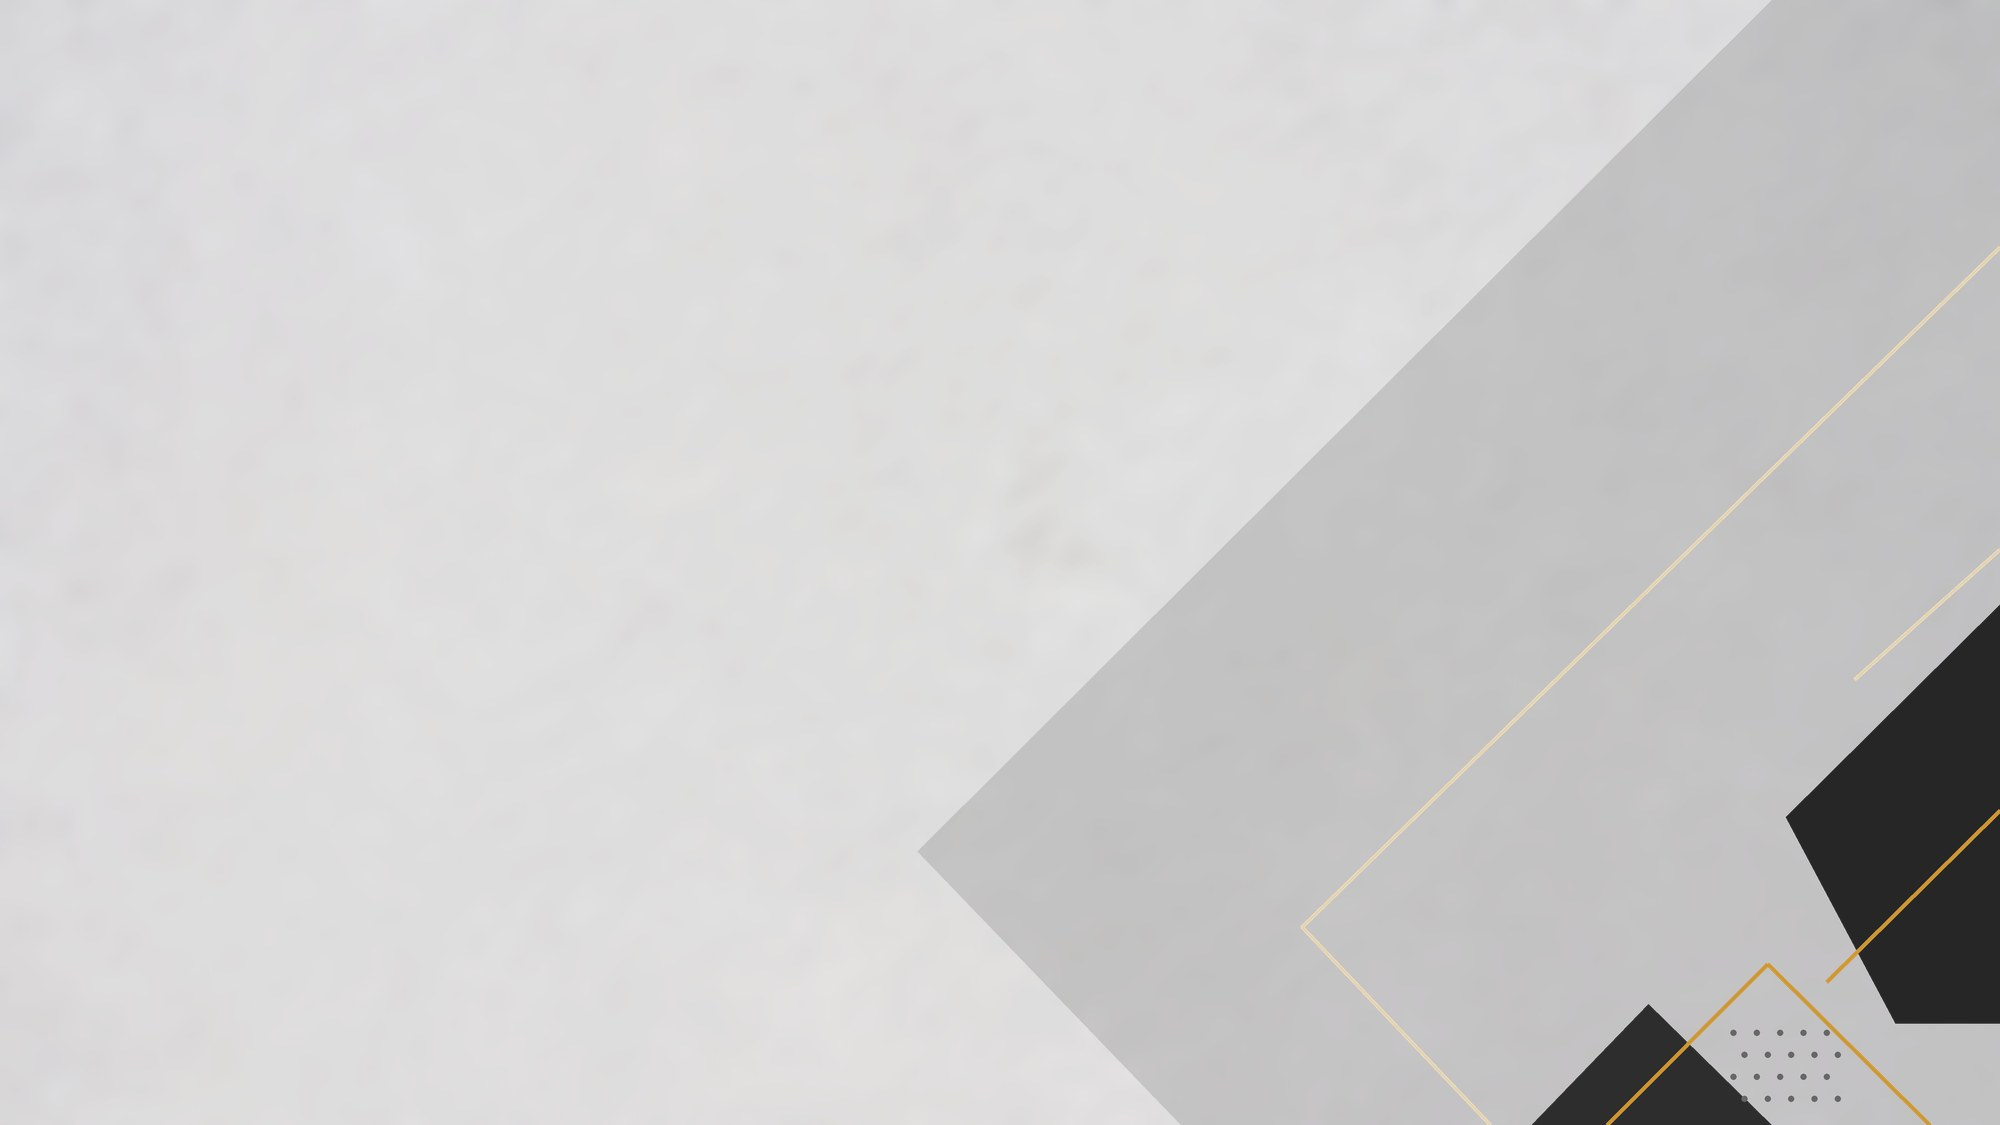
\includegraphics[width=1440bp,height=810bp]{../assets/template/bg_conteudo.jpg}};
  \end{tikzpicture}%
}

\newcommand{\ContentBox}[4]{%
  \begin{tikzpicture}[remember picture, overlay]
    \node[anchor=north west, inner sep=0bp]
      at ([xshift=#1, yshift=#2]current page.north west) {%
        \begin{minipage}[t]{#3}
          \raggedright
          #4\par
        \end{minipage}%
      };
  \end{tikzpicture}%
}

\newcommand{\sqbullet}{\raisebox{0.32ex}{\textcolor{InkBlack}{\rule{6.5bp}{6.5bp}}}}

\newenvironment{SlideList}[1][22bp]{%
  \begin{itemize}[leftmargin=24bp, label=\sqbullet, labelsep=12bp, itemsep=#1, topsep=0bp, parsep=0bp, partopsep=0bp]
}{%
  \end{itemize}%
}

\newenvironment{CompactList}[1][10bp]{%
  \begin{itemize}[leftmargin=20bp, label=\sqbullet, labelsep=10bp, itemsep=#1, topsep=0bp, parsep=0bp, partopsep=0bp]
}{%
  \end{itemize}%
}

\newcommand{\FigFrame}[2]{%
  \begin{tikzpicture}[baseline=(img.south)]
    \node[draw=CardBorder, line width=0.8bp, inner sep=4bp, fill=white] (img)
      {\includegraphics[width=#1]{#2}};
  \end{tikzpicture}%
}

\begin{document}

% ==============================================================================
% SLIDE 1 — CAPA (Integrante 1)
% ==============================================================================
\BgCover
\begin{tikzpicture}[remember picture, overlay]
  \node[anchor=north west, inner sep=0bp]
    at ([xshift=80bp, yshift=-170bp]current page.north west) {%
      \begin{minipage}[t]{890bp}
        \raggedright
        \fontsize{44bp}{54bp}\selectfont\bfseries\color{InkBlack}
        Análise Experimental de Indexação, Planos de Execução e Otimização de Consultas no Microsoft SQL Server 2022\par
      \end{minipage}%
    };
  \node[anchor=north west, inner sep=0bp]
    at ([xshift=80bp, yshift=-390bp]current page.north west) {%
      \begin{minipage}[t]{860bp}
        \raggedright
        \fontsize{21bp}{28bp}\selectfont\color{InkDark}
        Trabalho Final — Banco de Dados II \enspace\textbullet\enspace UFPI – CSHNB (Picos – PI)\par
      \end{minipage}%
    };
  \node[anchor=north west, inner sep=0bp]
    at ([xshift=80bp, yshift=-470bp]current page.north west) {%
      \begin{minipage}[t]{520bp}
        \raggedright
        \fontsize{21bp}{31bp}\selectfont\color{InkBlack}
        \textbf{Grupo:}\par
        Hermeson A.\par
        João Marcos R.\par
        Lizzandro W.\par
        Marcos W.\par
        Raildom R.\par
      \end{minipage}%
    };
  \draw[line width=2.2bp, color=black]
    ([xshift=80bp, yshift=-685bp]current page.north west) --
    ([xshift=480bp, yshift=-685bp]current page.north west);
  \node[anchor=south east, inner sep=0bp]
    at ([xshift=-48bp, yshift=40bp]current page.south east)
    {\fontsize{24bp}{28bp}\selectfont\color{white}1};
\end{tikzpicture}
\newpage

% ==============================================================================
% SLIDE 2 — INTRODUÇÃO, CONCEITOS E OBJETIVO (Integrante 1)
% ==============================================================================
\BgContent
\SlideTitle{Introdução e Fundamentação}
\SlideNumber{2}
\ContentBox{80bp}{-180bp}{960bp}{%
  \fontsize{24bp}{34bp}\selectfont\color{InkBlack}
  \begin{SlideList}[32bp]
    \item \textbf{Gargalo em escala:} varreduras integrais (\textit{Scan}) elevam E/S e disputam o \textit{buffer pool}, mesmo em SSDs.
    \item \textbf{Árvores B+ (8 KB):} busca $O(\log_m N)$ em 2–4 acessos; \texttt{INCLUDE} evita \textit{Key Lookup}, mas escritas pagam manutenção síncrona (\textit{write amplification}).
    \item \textbf{Otimizador e execução:} predicados sargáveis e \texttt{NOT EXISTS}; junções (\textit{Loops}, \textit{Merge}, \textit{Hash}) e \textit{Batch} vs. \textit{Row Mode}.
    \item \textbf{Objetivo:} medir ganhos e \textit{trade-offs} no \textbf{SQL Server 2022} em \textbf{6,25M linhas} (Q\textsubscript{1}–Q\textsubscript{10} e W\textsubscript{1}, \textit{Warm} e \textit{Cold}).
  \end{SlideList}
}
\newpage

% ==============================================================================
% SLIDE 3 — METODOLOGIA: AMBIENTE E BASES GÊMEAS (Integrante 2)
% ==============================================================================
\BgContent
\SlideTitle{Metodologia: Ambiente e Bases Gêmeas}
\SlideNumber{3}
\ContentBox{80bp}{-135bp}{900bp}{%
  \FigFrame{880bp}{../assets/tabelas/tabela1_print.png}
}
\ContentBox{80bp}{-495bp}{1020bp}{%
  \fontsize{20bp}{28bp}\selectfont\color{InkBlack}
  \begin{CompactList}[14bp]
    \item \textbf{Esquema B2C (\texttt{seed 42}, 400 MB):} \texttt{Clientes} (200k), \texttt{Produtos} (50k), \texttt{Pedidos} (1,5M) e \texttt{ItensPedido} (4,5M) = \textbf{6,25M linhas}.
    \item \textbf{Bases gêmeas (\texttt{BACKUP}/\texttt{RESTORE}):} \texttt{Baseline} (4 PKs clusterizadas) vs. \texttt{Otimizado} (+9 índices, amostragem 100\%).
    \item \textbf{Paridade garantida:} \texttt{sp\_updatestats}, FKs confiáveis (\texttt{is\_not\_trusted = 0}) e 12 estatísticas iniciais idênticas.
  \end{CompactList}
}
\newpage

% ==============================================================================
% SLIDE 4 — ÍNDICES IMPLANTADOS E PROTOCOLO (Integrante 2)
% ==============================================================================
\BgContent
\SlideTitle{Índices Secundários e Protocolo}
\SlideNumber{4}
\ContentBox{80bp}{-130bp}{840bp}{%
  \FigFrame{820bp}{../assets/tabelas/tabela2_print.png}
}
\ContentBox{80bp}{-592bp}{1040bp}{%
  \fontsize{18.5bp}{25bp}\selectfont\color{InkBlack}
  \begin{CompactList}[9bp]
    \item \textbf{Estratégias B+:} simples, cobertura (\texttt{INCLUDE}), composto \texttt{(Status, DataPedido)} e filtrado (\texttt{Desconto >= 10.00}).
    \item \textbf{Carga e controle:} 10 leituras + inserção de 10k itens (W\textsubscript{1} em \texttt{ROLLBACK}, 880 execuções) sob \texttt{MAXDOP 1}.
    \item \textbf{Regimes e estatística:} \textit{Warm} (N=30) vs. \textit{Cold} (N=10 pós-limpeza); Shapiro-Wilk $\rightarrow$ \textit{t} pareado ou Wilcoxon.
  \end{CompactList}
}
\newpage

% ==============================================================================
% SLIDE 5 — RESULTADOS EM WARM CACHE: TABELA 3 (Integrante 3)
% ==============================================================================
\BgContent
\SlideTitle{Resultados em Warm Cache (N = 30)}
\SlideNumber{5}
\ContentBox{80bp}{-135bp}{940bp}{%
  \FigFrame{920bp}{../assets/tabelas/tabela3_print.png}
}
\ContentBox{80bp}{-568bp}{1040bp}{%
  \fontsize{19bp}{26bp}\selectfont\color{InkBlack}
  \begin{CompactList}[10bp]
    \item \textbf{9/10 leituras ($p < 10^{-4}$):} maior ganho em Q\textsubscript{6} (\texttt{BACKWARD} sem \textit{Sort}: 8.090 $\rightarrow$ 3 págs, $>$424$\times$).
    \item \textbf{Sargabilidade:} prefixo em Q\textsubscript{8} (114,0$\times$) e intervalo semiaberto em Q\textsubscript{9} (8,69$\times$).
    \item \textbf{Contra-exemplos:} Q\textsubscript{7} eleva latência (0,60$\times$) e W\textsubscript{1} aumenta E/S em +85,33\%.
  \end{CompactList}
}
\newpage

% ==============================================================================
% SLIDE 6 — FIGURAS 1 E 2: E/S LÓGICA E LATÊNCIA (Integrante 3)
% ==============================================================================
\BgContent
\SlideTitle{E/S Lógica e Dispersão de Latência}
\SlideNumber{6}
\ContentBox{70bp}{-145bp}{535bp}{%
  \FigFrame{520bp}{../../paper/figures/fig1_leituras_logicas.png}
}
\ContentBox{615bp}{-145bp}{560bp}{%
  \FigFrame{545bp}{../../paper/figures/fig2_tempos_execucao_boxplot.png}
}
\ContentBox{80bp}{-430bp}{1030bp}{%
  \fontsize{20bp}{28bp}\selectfont\color{InkBlack}
  \begin{CompactList}[14bp]
    \item \textbf{Fig. 1 (E/S, escala log):} quedas de \textbf{99,58\%–99,96\%} em Q\textsubscript{1}–Q\textsubscript{4}, Q\textsubscript{6}; escrita W\textsubscript{1} sobe \textbf{+85,33\%} (97k $\rightarrow$ 180k págs).
    \item \textbf{Fig. 2a (OLTP):} consultas otimizadas estáveis em $\le$ 1,5 ms com dispersão mínima.
    \item \textbf{Fig. 2b (Junções e W\textsubscript{1}):} Q\textsubscript{5} (\textit{Merge + Loops}: 37,5$\times$) e Q\textsubscript{10} (\texttt{NOT EXISTS}: 1,69$\times$); W\textsubscript{1} varia amplamente ($\text{DP} = 853{,}2$ ms).
  \end{CompactList}
}
\newpage

% ==============================================================================
% SLIDE 7 — FIGURA 3: CASO Q4 E KEY LOOKUP (Integrante 4)
% ==============================================================================
\BgContent
\SlideTitle{Caso Q4: Eliminação de Key Lookup}
\SlideNumber{7}
\ContentBox{80bp}{-135bp}{920bp}{%
  \FigFrame{900bp}{../../paper/figures/fig3_q4_tres_estagios.png}
}
\ContentBox{80bp}{-622bp}{1030bp}{%
  \fontsize{19bp}{26bp}\selectfont\color{InkBlack}
  \begin{CompactList}[9bp]
    \item \textbf{1. Baseline:} \textit{Clustered Index Scan} — \textbf{8.090 págs} (\textbf{111,0 ms}).
    \item \textbf{2. Intermediário:} \textit{Index Seek} + \textbf{422 \textit{Key Lookups}} — \textbf{1.296 págs} (1,0 ms).
    \item \textbf{3. Otimizado (\texttt{INCLUDE}):} elimina \textit{Lookup} e \textit{Nested Loops} — \textbf{5 págs} (\textbf{$<$1 ms}, $-$99,94\%).
  \end{CompactList}
}
\newpage

% ==============================================================================
% SLIDE 8 — FIGURA 4: PLANOS FÍSICOS (.SQLPLAN) (Integrante 4)
% ==============================================================================
\BgContent
\SlideTitle{Planos Físicos de Execução (.sqlplan)}
\SlideNumber{8}
\ContentBox{80bp}{-132bp}{890bp}{%
  \FigFrame{870bp}{../../paper/figures/fig5_planos_execucao.pdf}
}
\ContentBox{80bp}{-665bp}{1050bp}{%
  \fontsize{18bp}{24bp}\selectfont\color{InkBlack}
  \begin{CompactList}[8bp]
    \item \textbf{(a–b) Busca e Cobertura:} Q\textsubscript{1} troca \textit{Scan} (2,329) por \textit{Seek + Lookup} (0,007); Q\textsubscript{4} remove \textit{Lookup} via \texttt{INCLUDE} (0,004).
    \item \textbf{(c–d) \textit{Trade-offs}:} Q\textsubscript{7} cai de \textit{Hash Match [Batch]} para \textit{Stream Aggregate [Row]}; W\textsubscript{1} grava em \textbf{4 árvores B+} (\textit{Sequence}).
  \end{CompactList}
}
\newpage

% ==============================================================================
% SLIDE 9 — TRADE-OFFS E COLD CACHE: FIGURA 5 (Integrante 5)
% ==============================================================================
\BgContent
\SlideTitle{Trade-offs e Cache: Warm vs. Cold}
\SlideNumber{9}
\ContentBox{80bp}{-135bp}{920bp}{%
  \FigFrame{900bp}{../../paper/figures/fig4_warm_vs_cold_cache.png}
}
\ContentBox{80bp}{-582bp}{1040bp}{%
  \fontsize{18.5bp}{25bp}\selectfont\color{InkBlack}
  \begin{CompactList}[9bp]
    \item \textbf{Inversão em Q\textsubscript{7} (\textit{Batch} $\rightarrow$ \textit{Row}):} $-$30,06\% E/S, mas latência sobe \textbf{217 $\rightarrow$ 364 ms} \textit{Warm} (0,60$\times$) e \textbf{402 $\rightarrow$ 685 ms} \textit{Cold} sob \texttt{MAXDOP 1}.
    \item \textbf{Escrita W\textsubscript{1} (4 B+ Trees):} +85,33\% E/S \textit{Warm} e \textbf{+264,73\%} \textit{Cold} (1.098,5 vs. 502,0 ms, 0,46$\times$; filtrado indexou 1.964 linhas).
    \item \textbf{\textit{Cold Cache} (N=10):} \texttt{physical\_reads >= 1} nas 220 execuções; leituras mantêm ganho (Q\textsubscript{1} 12,6$\times$; Q\textsubscript{5} 4,33$\times$).
  \end{CompactList}
}
\newpage

% ==============================================================================
% SLIDE 10 — CONCLUSÃO E REFERÊNCIAS (Integrante 5)
% ==============================================================================
\BgContent
\SlideTitle{Conclusão e Referências}
\SlideNumber{10}
\ContentBox{80bp}{-145bp}{1030bp}{%
  \fontsize{22bp}{29bp}\selectfont\bfseries\color{InkBlack}
  Conclusão e Limitações\par
  \vspace{6bp}
  \textcolor{GoldAccent}{\rule{1030bp}{2bp}}\par
  \vspace{14bp}
  \fontsize{19.5bp}{27bp}\selectfont\normalfont\color{InkBlack}
  \begin{CompactList}[12bp]
    \item \textbf{Ganhos expressivos em leitura:} até \textbf{$-$99,96\%} E/S (Q\textsubscript{6}), fim dos \textit{Key Lookups} (Q\textsubscript{4}) e aceleração em junções/sargabilidade (Q\textsubscript{5}, Q\textsubscript{8}, Q\textsubscript{9}).
    \item \textbf{Mais índices $\neq$ menor latência:} manutenção síncrona onera escrita (W\textsubscript{1} +85,33\%) e custo menor pode perder \textit{Batch Mode} (Q\textsubscript{7} +67,7\%).
    \item \textbf{Limitações:} execução serial (\texttt{MAXDOP 1}) em container único no mesmo SSD (sujeito ao cache do SO em \textit{Cold}).
  \end{CompactList}
}
\ContentBox{80bp}{-475bp}{1040bp}{%
  \fontsize{20bp}{26bp}\selectfont\bfseries\color{InkBlack}
  Referências\par
  \vspace{5bp}
  \textcolor{GoldAccent}{\rule{1040bp}{1.8bp}}\par
  \vspace{10bp}
  \fontsize{13.5bp}{19bp}\selectfont\normalfont\color{InkDark}
  \begin{CompactList}[5bp]
    \item Chaudhuri, S. (1998). \textit{An overview of query optimization in relational systems}. ACM PODS, p. 34–43.
    \item Comer, D. (1979). \textit{The ubiquitous B-tree}. ACM Computing Surveys, 11(2):121–137.
    \item Elmasri, R.; Navathe, S. B. (2016). \textit{Fundamentals of Database Systems}. Pearson, 7th ed.
    \item Graefe, G. (1993). \textit{Query evaluation techniques for large databases}. ACM Computing Surveys, 25(2):73–169.
    \item Microsoft Corporation (2022). \textit{Query processing architecture guide – SQL Server 2022}. Microsoft Learn.
    \item Ramakrishnan, R.; Gehrke, J. (2003). \textit{Database Management Systems}. McGraw-Hill, 3rd ed.
    \item Selinger, P. G. et al. (1979). \textit{Access path selection in a relational DBMS}. ACM SIGMOD, p. 23–34.
    \item Silberschatz, A.; Korth, H. F.; Sudarshan, S. (2020). \textit{Database System Concepts}. McGraw-Hill, 7th ed.
  \end{CompactList}
}

\end{document}
